\documentclass{article}
\usepackage{tikz}
\usetikzlibrary{positioning, decorations.pathreplacing}

\begin{document}

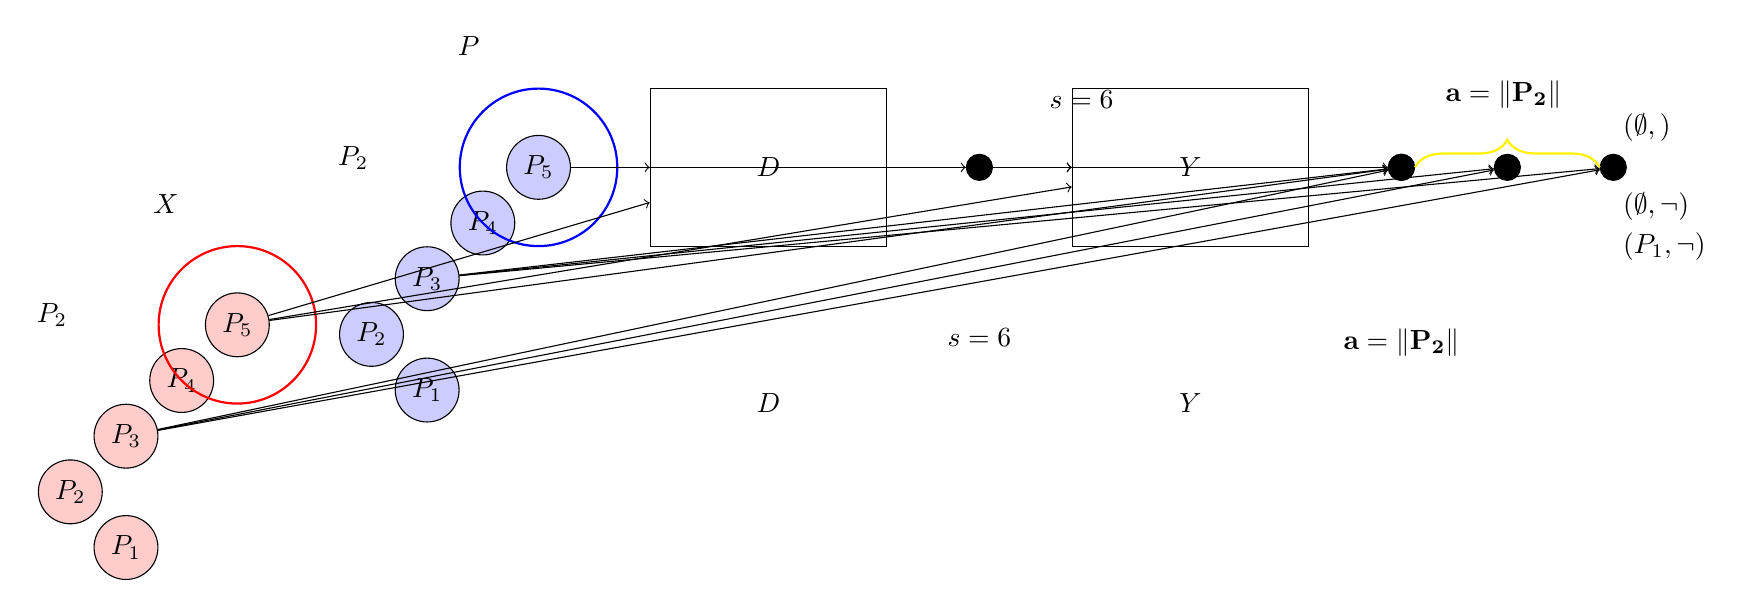
\begin{tikzpicture}[node distance=1cm, auto]
    % Define nodes for the circles
    \node (P) [circle, draw, fill=blue!20] {$P_5$};
    \node (P1) [below left of=P, circle, draw, fill=blue!20] {$P_4$};
    \node (P2) [below left of=P1, circle, draw, fill=blue!20] {$P_3$};
    \node (P3) [below left of=P2, circle, draw, fill=blue!20] {$P_2$};
    \node (P4) [below right of=P3, circle, draw, fill=blue!20] {$P_1$};
    
    \node (X) [left=of P, xshift=-2cm, yshift=-2cm, circle, draw, fill=red!20] {$P_5$};
    \node (X1) [below left of=X, circle, draw, fill=red!20] {$P_4$};
    \node (X2) [below left of=X1, circle, draw, fill=red!20] {$P_3$};
    \node (X3) [below left of=X2, circle, draw, fill=red!20] {$P_2$};
    \node (X4) [below right of=X3, circle, draw, fill=red!20] {$P_1$};
    
    % Draw the circles
    \draw[thick, red] (X) circle (1);
    \draw[thick, blue] (P) circle (1);
    
    % Define nodes for the diagram
    \node (D) [right=of P, rectangle, draw, minimum width=3cm, minimum height=2cm] {$D$};
    \node (s) [right=of D, circle, draw, fill=black] {};
    \node (s_label) [right=of s, label={[label distance=0.5cm]above:$s=6$}] {};
    \node (Y) [right=of s, rectangle, draw, minimum width=3cm, minimum height=2cm] {$Y$};
    \node (a) [right=of Y, circle, draw, fill=black] {};
    \node (a_label) [right=of a, label={[label distance=0.5cm]above:$\mathbf{a}=\mathbf{\|P_2\|}$}] {};
    
    % Draw the connections
    \draw[->] (D) -- (s);
    \draw[->] (s) -- (Y);
    
    % Define nodes for the labels
    \node (P_label) [above=of P, label={[label distance=0.5cm]left:$P$}] {};
    \node (X_label) [above=of X, label={[label distance=0.5cm]left:$X$}] {};
    \node (D_label) [below=of D, label={[label distance=0.5cm]below:$D$}] {};
    \node (s_label) [below=of s, label={[label distance=0.5cm]below:$s=6$}] {};
    \node (Y_label) [below=of Y, label={[label distance=0.5cm]below:$Y$}] {};
    \node (a_label) [below=of a, label={[label distance=0.5cm]below:$\mathbf{a}=\mathbf{\|P_2\|}$}] {};
    
    % Define nodes for the annotations
    \node (annotation1) [right=of Y, circle, draw, fill=black] {};
    \node (annotation2) [right=of annotation1, circle, draw, fill=black] {};
    \node (annotation3) [right=of annotation2, circle, draw, fill=black] {};
    
    % Draw the annotations
    \draw[decorate, decoration={brace, amplitude=10pt}, thick, color=yellow] (annotation1) -- (annotation3);
    \node at (annotation1 -| annotation3) [above=0.5cm, anchor=west] {$(\emptyset,\square)$};
    \node at (annotation1 -| annotation3) [below=0.5cm, anchor=west] {$(\emptyset,\neg\square)$};
    \node at (annotation1 -| annotation3) [below=1cm, anchor=west] {$(P_1,\neg\square)$};
    
    % Define nodes for the labels
    \node (P2_label) [above=of P2, label={[label distance=0.5cm]left:$P_2$}] {};
    \node (P2_label) [above=of X2, label={[label distance=0.5cm]left:$P_2$}] {};
    
    % Draw the connections
    \draw[->] (P) -- (D);
    \draw[->] (P) -- (Y);
    \draw[->] (P) -- (a);
    
    \draw[->] (X) -- (D);
    \draw[->] (X) -- (Y);
    \draw[->] (X) -- (a);
    
    \draw[->] (P2) -- (annotation1);
    \draw[->] (P2) -- (annotation2);
    \draw[->] (P2) -- (annotation3);
    
    \draw[->] (X2) -- (annotation1);
    \draw[->] (X2) -- (annotation2);
    \draw[->] (X2) -- (annotation3);
    
\end{tikzpicture}

\end{document}